% \cleardoublepage
\chapter{Contribution 2}\label{sec:contrib2}\minitoc\vspace{.5cm}
\index{Contribution 2}

\section{Introduction}

\begin{wrapfigure}{r}{0.2\textwidth}
    \centering
    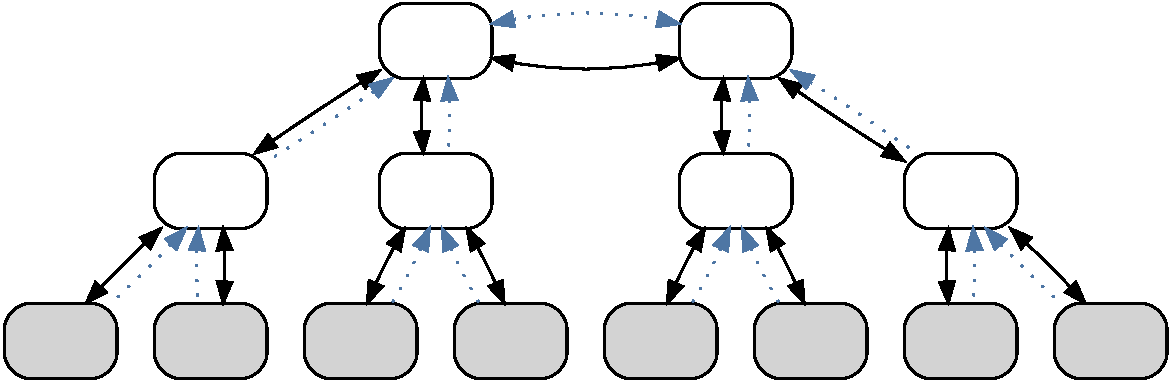
\includegraphics[width=0.2\textwidth]{resources/images/example3}
\end{wrapfigure}

\sidenote{Overview}
\todomid{write}

\sidenote{Structure of Research}
\todomid{write about \Cref{fig:hourglass:contrib2}}

\begin{figure}[H]
    \centering
    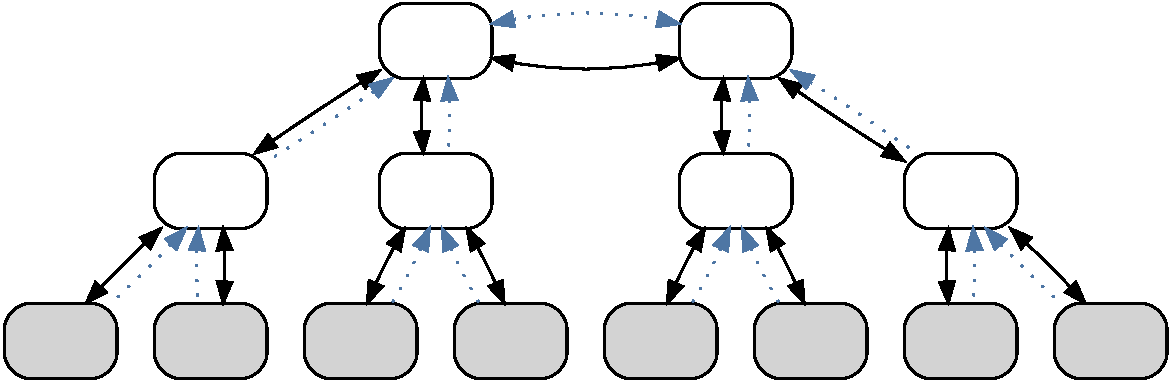
\includegraphics[width=.55\textwidth]{resources/images/example3}
    \caption{Placement of Contribution 2 in the structure of research}\label{fig:hourglass:contrib2}
\end{figure}

\section{State of the Art}

\sidenote{Overview}
\todomid{write about \Cref{fig:contrib2:related}}

\begin{figure}[htbp]
    \centering
    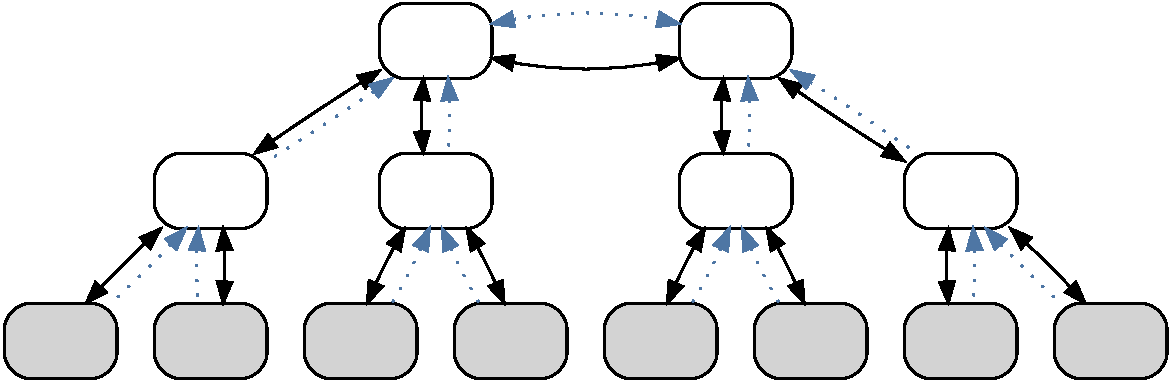
\includegraphics[width=.6\textwidth]{resources/images/example3}
    \caption{Relationship of Contribution 2 to related work}\label{fig:contrib2:related}
\end{figure}

\subsection{Related Work 1}

\sidenote{Overview}
\todomid{write}

\sidenote{Some Aspects}
\todomid{write}

\sidenote{Issues}
\todomid{write about \Cref{lst:contrib2:rw1}}

\lstset{caption=Listing related to related work 1 for Contribution 2, label=lst:contrib2:rw1,
language=xml, breaklines=true, numbers=left, basicstyle=\small\ttfamily,
stepnumber=1, frame=single, inputencoding=utf8/latin1}~\lstinputlisting{resources/code/example.java}

\subsection{Related Work 2}

\sidenote{Overview}
\todomid{write}

\sidenote{Some Aspects}
\todomid{write}

\sidenote{Issues}
\todomid{write about \Cref{lst:contrib2:rw2}}

\lstset{caption=Listing related to related work 2 for Contribution 2, label=lst:contrib2:rw2,
language=xml, breaklines=true, numbers=left, basicstyle=\small\ttfamily,
stepnumber=1, frame=single, inputencoding=utf8/latin1}~\lstinputlisting{resources/code/example.java}

\subsection{Related Work 3}

\sidenote{Overview}
\todomid{write}

\sidenote{Some Aspects}
\todomid{write}

\sidenote{Issues}
\todomid{write about \Cref{lst:contrib2:rw3}}

\lstset{caption=Listing related to related work 3 for Contribution 2, label=lst:contrib2:rw3,
language=xml, breaklines=true, numbers=left, basicstyle=\small\ttfamily,
stepnumber=1, frame=single, inputencoding=utf8/latin1}~\lstinputlisting{resources/code/example.java}


\section{Own Approach}

\subsection{Overview}

\sidenote{Intro}
\todomid{write}

\sidenote{Goal}
\todomid{write about \Cref{fig:contrib2:goal}}

\begin{figure}[htbp]
    \centering
    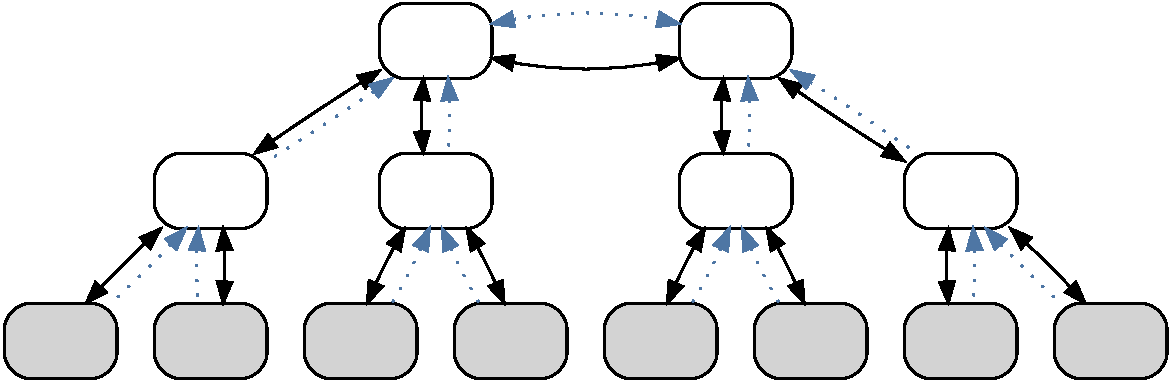
\includegraphics[width=.95\textwidth]{resources/images/example3}
    \caption{Contribution 2 goal}\label{fig:contrib2:goal}
\end{figure}

\sidenote{Approach}
\todomid{write}

\subsection{First Part}

\sidenote{Overview}
\todomid{write}

\sidenote{Approach}
\todomid{write}

\sidenote{Integration}
\todomid{write}

\subsection{Second Part}

\sidenote{Overview}
\todomid{write}

\sidenote{Approach}
\todomid{write}

\sidenote{Integration}
\todomid{write}

\subsection{Third Part}

\sidenote{Overview}
\todomid{write}

\sidenote{Approach}
\todomid{write}

\sidenote{Integration}
\todomid{write}

\section{Conclusion}

\sidenote{Summary}
\todomid{write}

\sidenote{Takeaway 1}
\todomid{write}

\sidenote{Takeaway 2}
\todomid{write}

\sidenote{Takeaway 3}
\todomid{write}

\sidenote{Next chapter}
\todomid{write}
